\documentclass{article}

\usepackage[a4paper,margin=1in]{geometry}
\usepackage{fancyhdr}
\usepackage{amsmath}
\usepackage{booktabs}
\usepackage{listings}
\usepackage{graphicx}
\usepackage{asymptote}

\pagestyle{fancy}
\fancyhf{}
\lhead{Programming Language: Assignment 3}
\rhead{Sui Qingyu (5090309011)}
\cfoot{\thepage}

\setlength\parskip{0.5em}

\lstset{numbers=left,
        numberstyle=\scriptsize,
        frame=lines,
        flexiblecolumns=false,
        language=C,
        basicstyle=\ttfamily\small,
        breaklines=true,
        extendedchars=true,
        escapechar=\%,
        texcl=true,
        showstringspaces=true,
        keywordstyle=\bfseries,
        tabsize=4}

\begin{document}
\section*{Problem 1}
\textbf{Q:} \textit{For the listed languages, list all the basic types supported, and write a program to get the size, in bytes, of each type: C++, Java, Pascal.}

The types and their size for these 3 languages are shown in Table \ref{t:cpptype}, \ref{t:javatype} and \ref{t:pascaltype}.

Notice that because there are too many types in Freepascal, I ignored some types like ``wordbool''.

\begin{table}[hp]
\centering
\begin{tabular}{ccl}
\toprule
Type & Size (byte) & \multicolumn{1}{c}{Note} \\
\midrule
void & 0 & Special type, which means ``no type''. \\
bool & 1 & Boolean type with value ``true'' or ``false''. \\
{[signed]} short {[int]} & 2 & Integer from $-2^{15}$ to $2^{15}-1$. \\
unsigned short {[int]} & 2 & Integer from $0$ to $2^{16}-1$. \\
signed {[int]} / int & 4 & Integer from $-2^{31}$ to $2^{31}-1$. \\
unsigned {[int]} & 4 & Integer from $0$ to $2^{32}-1$. \\
{[signed]} long {[int]} & 4 & Same as ``signed int''. \\
unsigned long {[int]} & 4 & Same as ``unsigned int''. \\
{[signed]} long long {[int]} & 8 & Integer from $-2^{63}$ to $2^{63}-1$. \\
unsigned long long {[int]} & 8 & Integer from $0$ to $2^{64}-1$. \\
{[signed]} char & 1 & Character with code from $-2^7$ to $2^7-1$. \\
unsigned char & 1 & Character with code from $0$ to $2^8-1$. \\
wchar\_t & 2 & Character with code from $0$ to $2^{16}-1$. \\
float & 4 & Single precision float. \\
double & 8 & Double precision float. \\
long double & 8 & Same as ``double''. \\
\bottomrule
\end{tabular}
\caption{Types in C++}
\label{t:cpptype}
\end{table}

\begin{table}[hp]
\centering
\begin{tabular}{ccl}
\toprule
Type & Size (byte) & \multicolumn{1}{c}{Note} \\
\midrule
byte & 1 & Integer from $-2^7$ to $2^7-1$. \\
short & 2 & Integer from $-2^{15}$ to $2^{15}-1$. \\
int & 4 & Integer from $-2^{31}$ to $2^{31}-1$. \\
long & 8 & Integer from $-2^{63}$ to $2^{63}-1$. \\
float & 4 & Single precision float. \\
double & 8 & Double precision float. \\
char & 2 & Character with code from $0$ to $2^{16}-1$. \\
boolean & 1 & Boolean type with value ``true'' or ``false''. \\
\bottomrule
\end{tabular}
\caption{Types in Java}
\label{t:javatype}
\end{table}

\begin{table}[hp]
\centering
\begin{tabular}{ccl}
\toprule
Type & Size (byte) & \multicolumn{1}{c}{Note} \\
\midrule
shortint & 1 & Integer from $-2^7$ to $2^7-1$. \\
smallint / integer & 2 & Integer from $-2^{15}$ to $2^{15}-1$. \\
longint & 4 & Integer from $-2^{31}$ to $2^{31}-1$. \\
int64 & 8 & Integer from $-2^{63}$ to $2^{63}-1$. \\
byte & 1 & Integer from $0$ to $2^8-1$. \\
word & 2 & Integer from $0$ to $2^{16}-1$. \\
cardinal / longword & 4 & Integer from $0$ to $2^{32}-1$. \\
qword & 8 & Integer from $0$ to $2^{64}-1$. \\
single & 4 & Single precision float. \\
real / double & 8 & Double precision float. \\
extended & 10 & Float with wider range and significant bits than ``double''. \\
comp & 8 & Float with wider significant bits, but less range than ``double''. \\
currency & 8 & Float with wider significant bits, but less range than ``comp''. \\
boolean & 1 & Boolean type with value ``true'' or ``false''. \\
char & 1 & Character with code from $0$ to $2^8-1$. \\
string & maximum 255 & String type. \\
ansistring & unlimited & Longer string type. \\
\bottomrule
\end{tabular}
\caption{Types in Pascal (Free Pascal)}
\label{t:pascaltype}
\end{table}

\section*{Problem 4}
\textbf{Q:} \textit{Define an EBNF and abstract syntax for records structures in Clite. The EBNF for structure references should use the “dot” notation discussed in the class. Modify the Clite project, the Lexer and the Parser, to make it parse a structure.}

The EBNF for structure is:

\begin{align*}
Structure &\rightarrow Structure\ .\ Identifier\ |\ Identifier \\
Identifier &\rightarrow Letter\ \{\ Letter\ |\ Digit\ \} \\
Letter &\rightarrow \mathrm{a}\ |\ \mathrm{b}\ | \dots |\ \mathrm{z}\ |\ \mathrm{A}\ |\ \mathrm{B}\ | \dots |\ \mathrm{Z} \\
Digit &\rightarrow 0\ |\ 1\ | \dots |\ 9
\end{align*}

\section*{Problem 6}
\textbf{Q:} \textit{For each of the following statements using the implicit typing rules of Section 6.1, first draw the untyped abstract syntax tree, then add type information, as done in Section 6.2. If any typed abstract syntax tree is invalid, clearly indicate where and why.}

The abstract syntax tree are shown in Figure \ref{p:6a}, \ref{p:6b}, \ref{p:6c}, \ref{p:6d} and \ref{p:6e}.

As we see, in Fiture \ref{p:6b}, the last assignment is not valid because it's putting a float value into an integer varible.

\begin{figure}[hp]
\centering
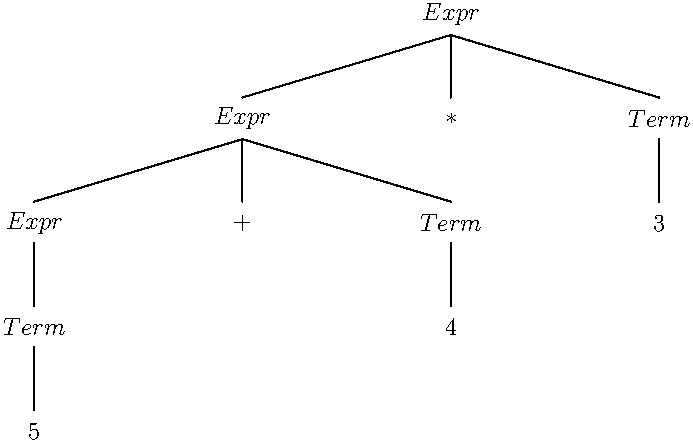
\includegraphics{p1.pdf}
\caption{Abstract syntax tree for ``f = -3;''}
\label{p:6a}
\end{figure}

\begin{figure}[hp]
\centering
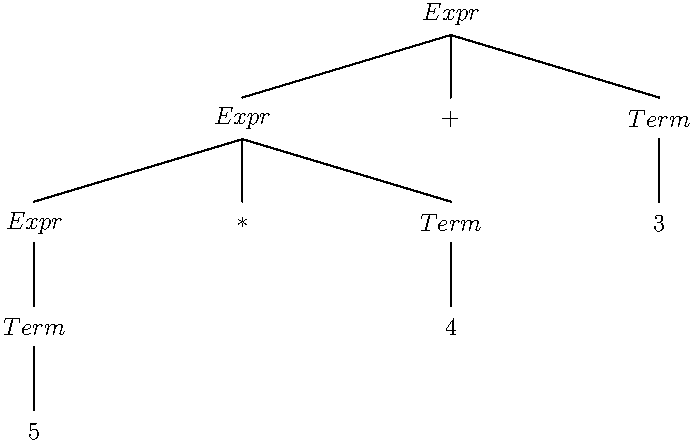
\includegraphics{p2.pdf}
\caption{Abstract syntax tree for ``i = -2.5;''}
\label{p:6b}
\end{figure}

\begin{figure}[hp]
\centering
\includegraphics{p3.pdf}
\caption{Abstract syntax tree for ``i = c;''}
\label{p:6c}
\end{figure}

\begin{figure}[hp]
\centering
\includegraphics{p4.pdf}
\caption{Abstract syntax tree for ``f = f + 1;''}
\label{p:6d}
\end{figure}

\begin{figure}[hp]
\centering
\includegraphics{p5.pdf}
\caption{Abstract syntax tree for ``if (f1 > f2) f3 = f4 + f5;''}
\label{p:6e}
\end{figure}

\section*{Problem 7}
\textbf{Q:} \textit{Show that the integer type can be defined as a recursive type starting with just the value null. Then write a function that checks if two integers defined in this way are equal.}

Here comes the definition:

\begin{lstlisting}
struct IntBase
{
    IntBase *next;
};

typedef IntBase* Int;
\end{lstlisting}

Then we use type ``Int'' to represent an integer. If an ``Int foo'' equals to null, then the value of foo is zero. And if foo-$>$next equals to null, the value equals to 1. The rest may be deduced by analogy.

A equalize checking function is shown below:

\begin{lstlisting}
bool IntEqual(Int a, Int b)
{
    while (a != NULL && b != NULL)
    {
        a = a->next;
        b = b->next;
    }
    return a == b;
}
\end{lstlisting}

\section*{Problem 9}
\textbf{Q:} \textit{Finish the rest of the typing rules for L\{num-str\} on lecture slide \#36.}

\begin{align*}
\frac{G \vdash e_1: num\ \ G \vdash e_2: num}{G \vdash assignment(e_1; e_2): num} \\
\frac{G \vdash e_1: string\ \ G \vdash e_2: string}{G \vdash assignment(e_1; e_2): string}
\end{align*}

\section*{Problem 10}
\textbf{Q:} \textit{Prove by induction the ``weakening lemma'' w.r.t. the L\{num-str\} language and its typing rules.}

\begin{equation*}
\displaystyle{\frac{\frac{}{G \vdash e': t'}\ \ \frac{}{G, x: t \vdash x: t}}{G, x: t \vdash e': t'}}
\end{equation*}

\end{document}


